\section{ELEMENT TACTICS}
\label{sec:ttp_aa:tactics_element}

\paragraph{Element}
The fundamental unit in A-A tactics is the two-ship lead-wingman combination.
Allows mutual support and protection within element

\subsection{ELEMENT RESPONSIBILITIES}

\paragraph{Lead}
\begin{itemize}
    \item tactics / flow
    \item risk management
    \item higher-level planning \& communication
\end{itemize}

\paragraph{Wingman}
\begin{itemize}
    \item maintain formation
    \item sensors
    \item communication with lead
\end{itemize}

\subsection{SENSORS \& SORT}

\paragraph{Pre-Commit Search}
\begin{itemize}
    \item \textbf{Element lead} --- high, search volume from contrails down at desired range
    \item \textbf{Wingman} --- low, search volume from ground up at desired range
\end{itemize}
\paragraph{Standard Sort}
\begin{itemize}
    \item \textbf{Element lead} --- side / high / near
    \item \textbf{Wingman} --- side / low / far
\end{itemize}
\hfill(unless otherwise briefed)

\clearpage

\subsection{OFFENSIVE TACTICS}

\paragraph{Intercept Timelines} 
\Cref{sec:ttp_aa:timelines} extends directly to a two-ship:
\begin{itemize}
    \item increased targeting capacity
    \item increased opportunities for mutual support
\end{itemize}

\paragraph{Notch-Press}
Employment of launch-and-decide banzai tactics, 
reference \cref{subsec:ttp_aa:timeline:banzai},
as an element. Lead, wingman notch in opposite directions, 
spiked fighter aborts, 
naked fighter presses.

\begin{multicols}{2}
    \textbf{Advantages}
    \begin{itemize}
        \item increases chance of at least 1 fighter being naked
        \item maximizes geometric problem for bandit
        \item impedes bandit radar lock
    \end{itemize}
    \columnbreak
    \textbf{Disadvantages}
    \begin{itemize}
        \item if bandit equipped with active-radar missiles may not get spiked even if targeted
        \item multiple bandits can sort, spiking both fighters
    \end{itemize}
\end{multicols}

\hfill\textbf{see \cref{fig:ttp_aa:element:offensive:notchpress}}

\begin{figure}[htbp]
    \centering
    \begin{tikzpicture}[figstyle]

        % coordinates
        \coordinate (naked_start) at (5,0);
        \coordinate (spiked_start) at (-5,0);
        \coordinate (bandit) at (0,60);

        \coordinate (naked_notch_start) at (5,15);
        \coordinate (spiked_notch_start) at (-5,15);

        % bandit wez
        \draw[fill=red!40]
            (bandit)
            -- ++(-110:48)
            arc (-110:-120:48)
            -- (bandit);

        \node[rotate=-90] (naked_notch_mid) at (20, 20) {
            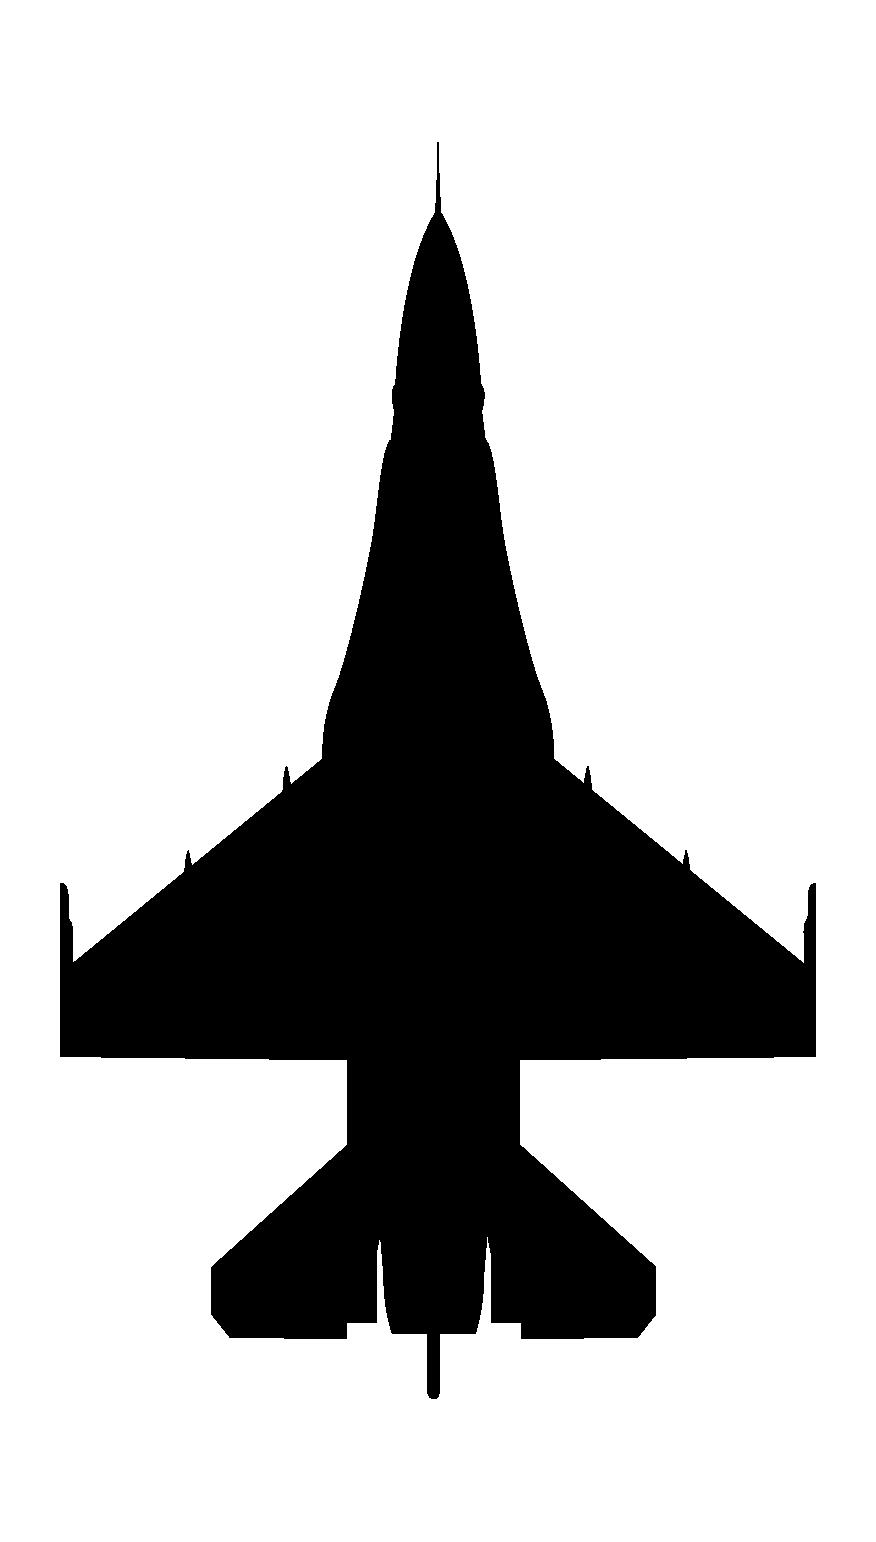
\includegraphics[
                width=7.5mm,
            ]{diagrams/aircraft/silhouette_f16_top.pdf}
        };
        \node[rotate=90] (spiked_notch_mid) at (-20, 20) {
            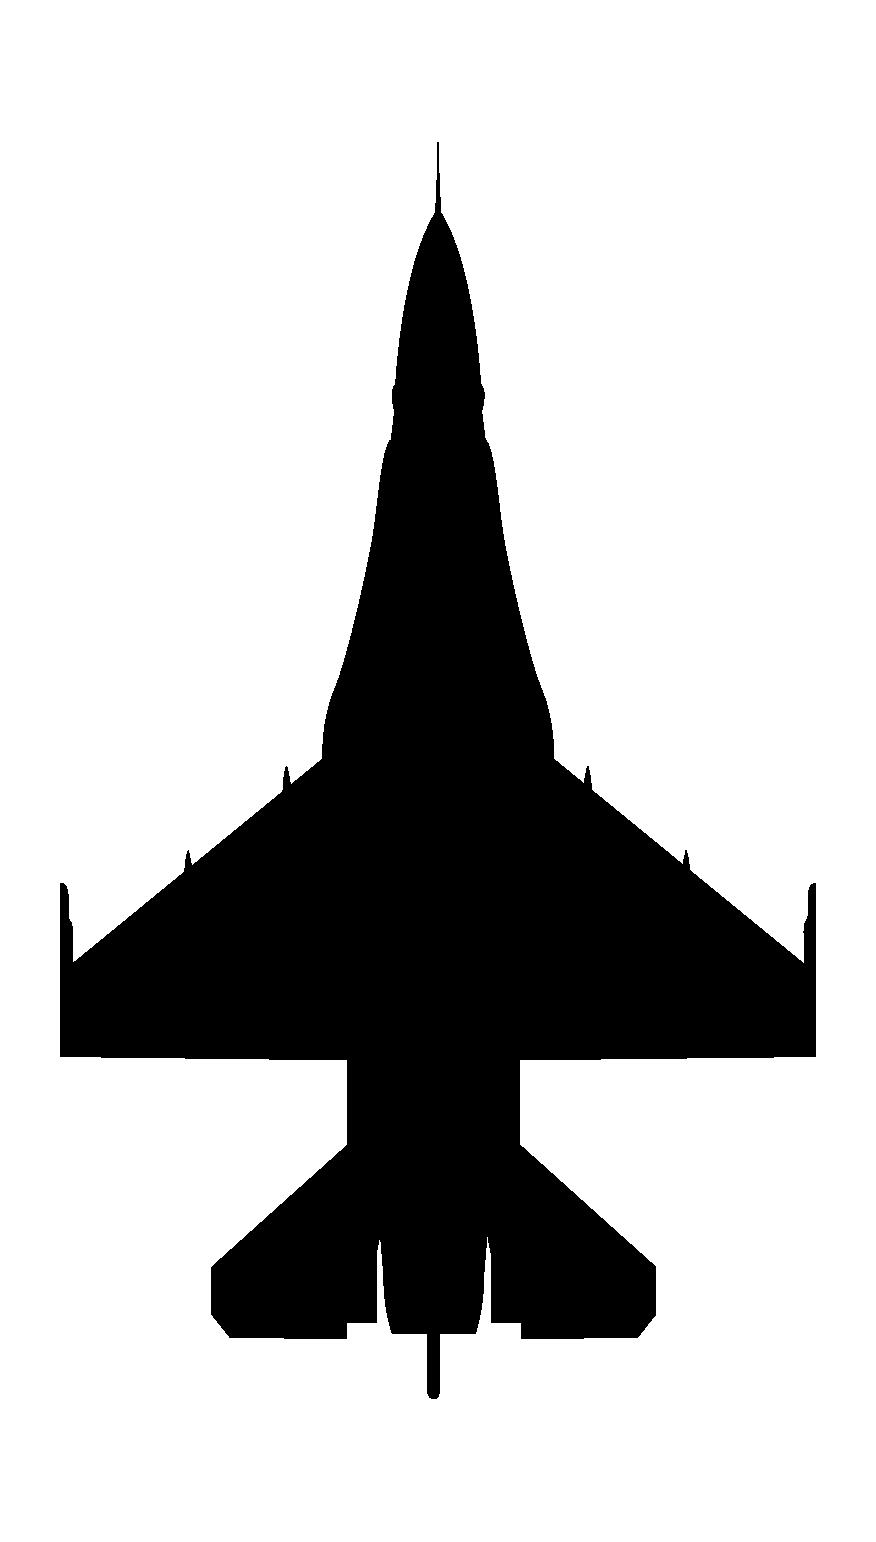
\includegraphics[
                width=7.5mm,
            ]{diagrams/aircraft/silhouette_f16_top.pdf}
        };
        
        % naked fighter
        \draw[->] 
            (naked_start) -- 
            node[below, pos=0]{
                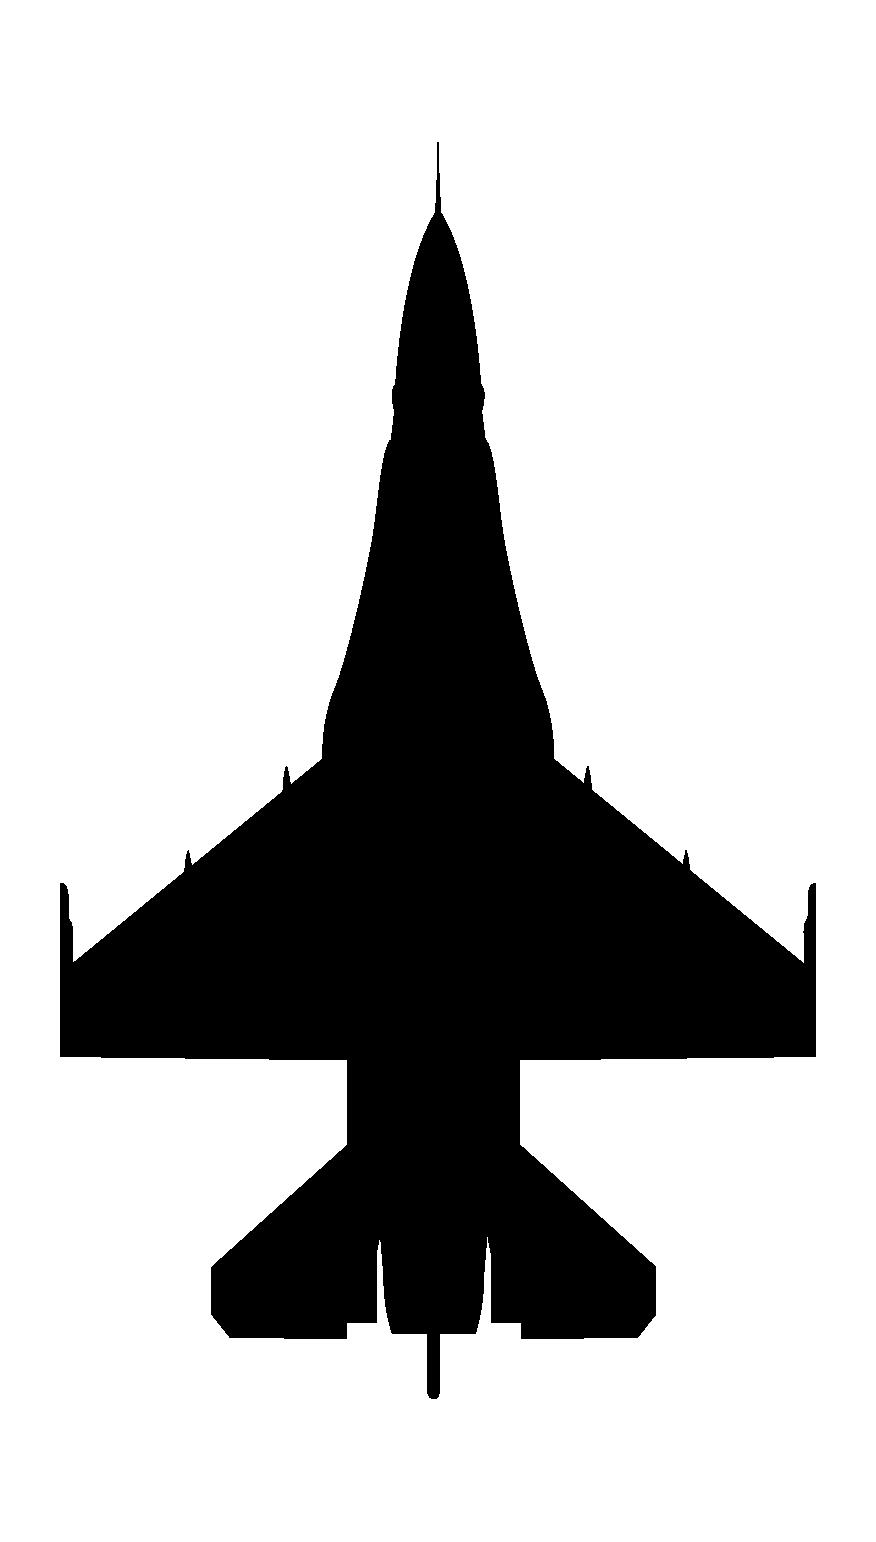
\includegraphics[
                width=7.5mm,
            ]{diagrams/aircraft/silhouette_f16_top.pdf}} 
            (naked_notch_start)
            arc (180:90:5) 
            -- (naked_notch_mid);
        \draw[->]
            (naked_notch_mid.north)
            arc (-90:45:5) 
            -- ++(135:10)
            node[above, pos=1, rotate=45] (naked_commit) {
                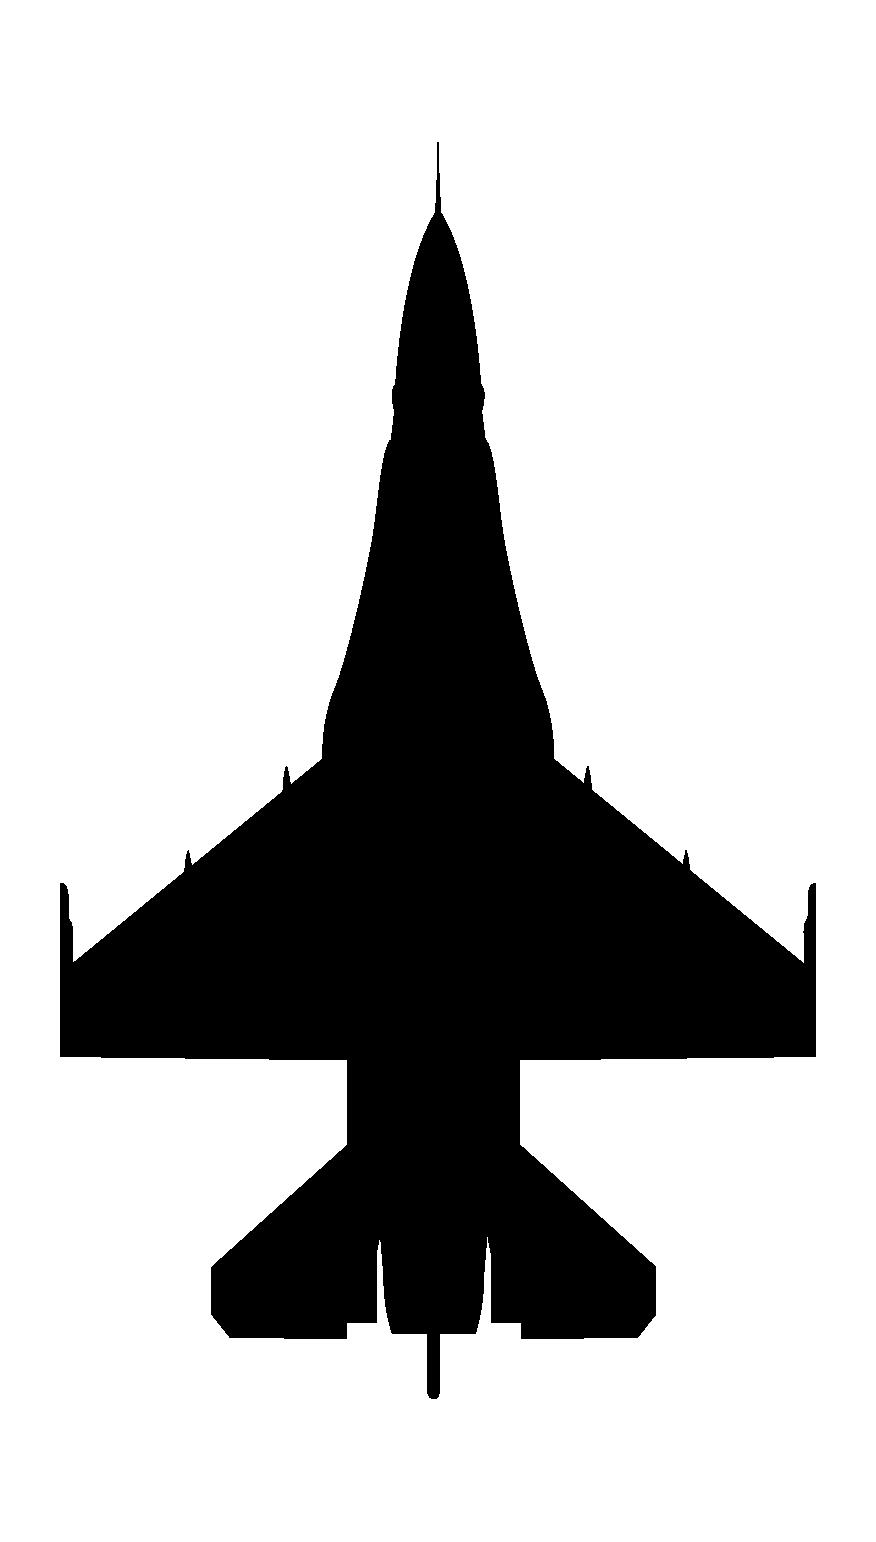
\includegraphics[
                    angle=0,
                    width=7.5mm,
            ]{diagrams/aircraft/silhouette_f16_top.pdf}};

        \node[font=\footnotesize, below] at (naked_notch_mid.east) {Naked}; 
        \node[font=\footnotesize, right] at (naked_commit.east) {Commit};

        % spiked fighter
        \draw[->] 
            (spiked_start) -- 
            node[below, pos=0]{
                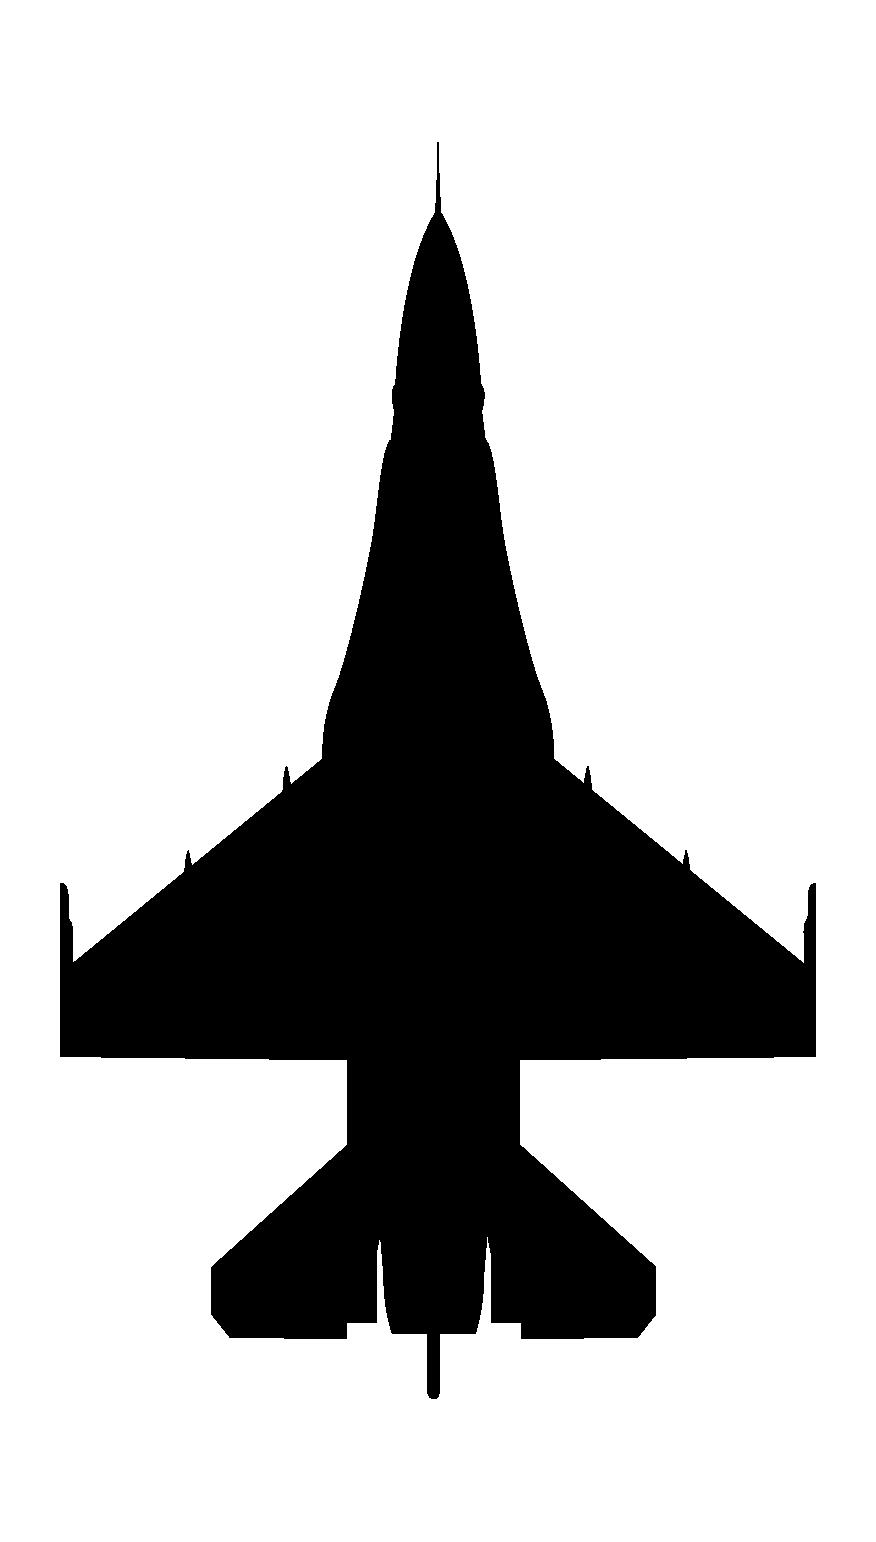
\includegraphics[
                width=7.5mm,
            ]{diagrams/aircraft/silhouette_f16_top.pdf}} 
            (spiked_notch_start)
            arc (0:90:5) 
            -- (spiked_notch_mid);
        \draw[->]
            (spiked_notch_mid.north)
            arc (90:180:5) 
            -- ++(0,-10)
            node[below, pos=1] (spiked_abort) {
                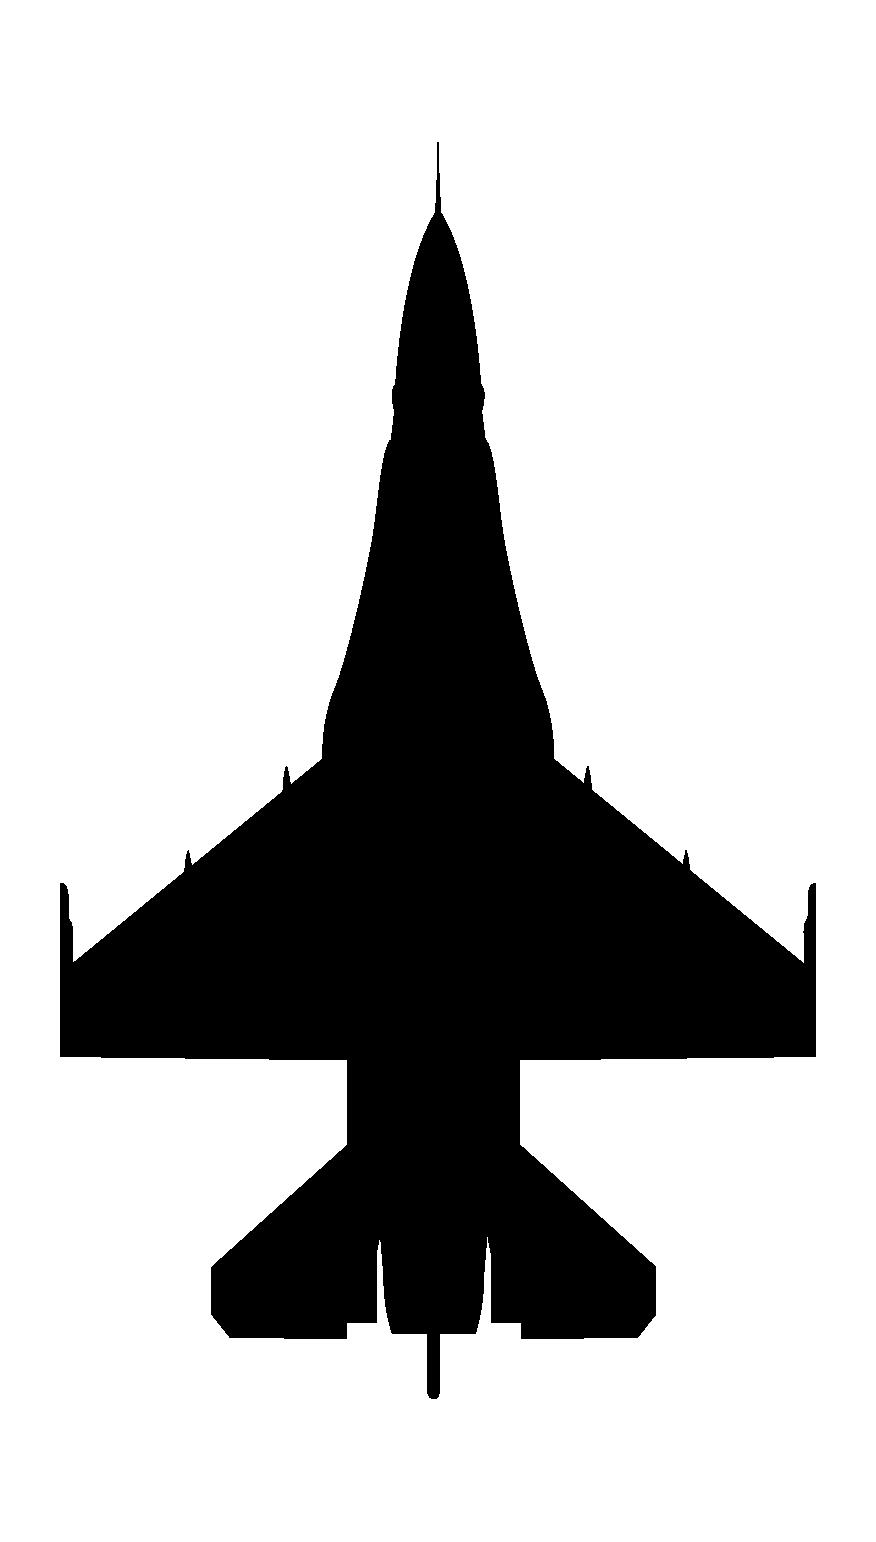
\includegraphics[
                    angle=180,
                    width=7.5mm,
            ]{diagrams/aircraft/silhouette_f16_top.pdf}};

        \node[font=\footnotesize, below] at (spiked_notch_mid.west) {Spiked}; 
        \node[font=\footnotesize, below] at (spiked_abort.south) {Abort};

        % bandit
        \node[] at (bandit) {
            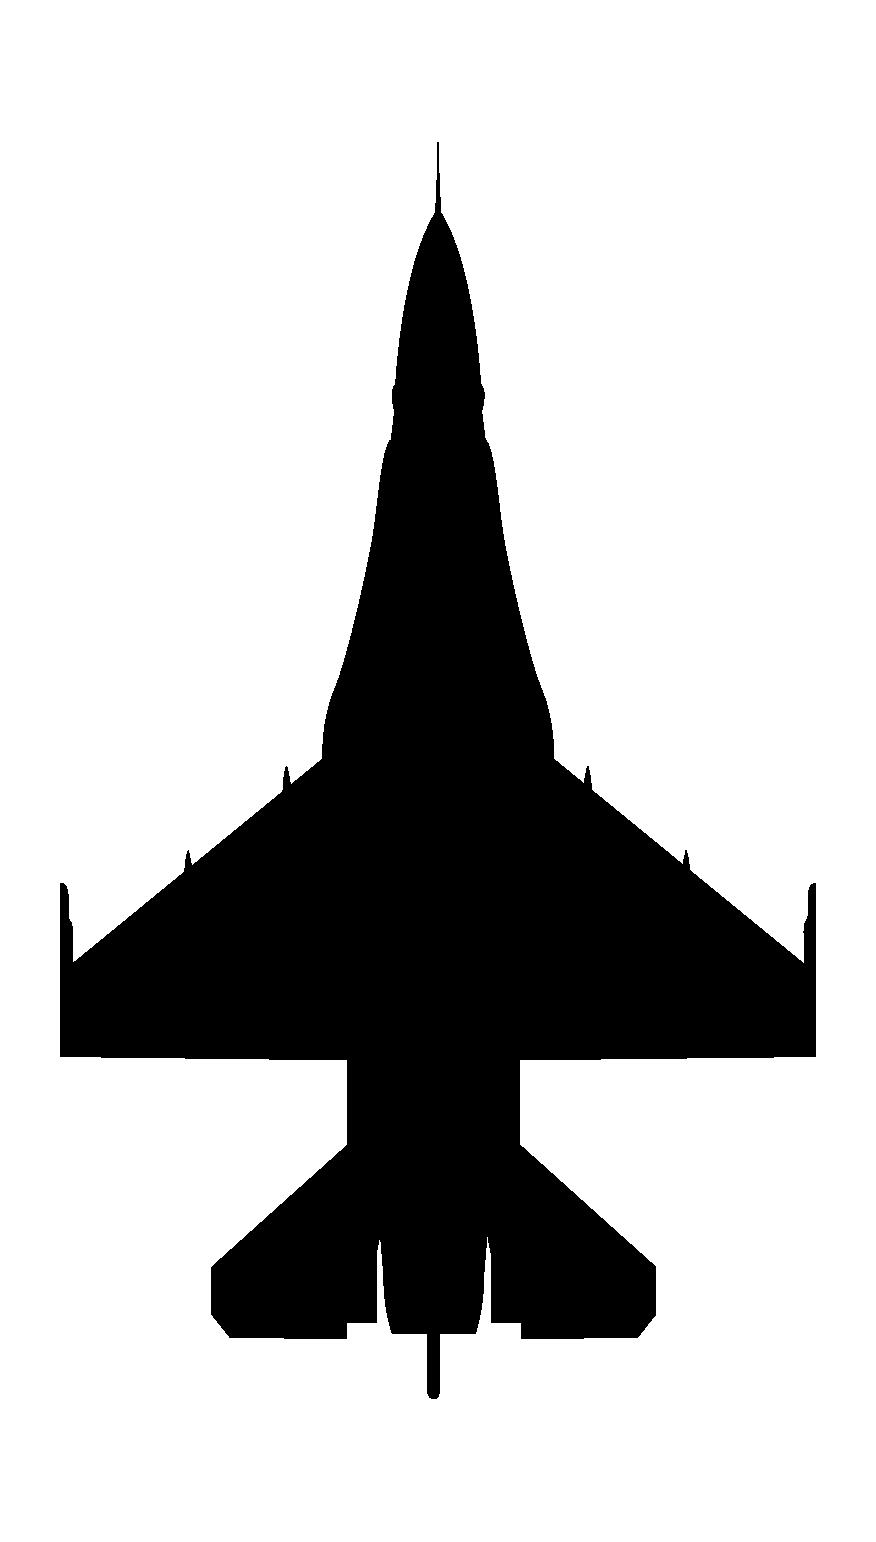
\includegraphics[
                angle=180,
                width=7.5mm,
        ]{diagrams/aircraft/silhouette_f16_top.pdf}};

    \end{tikzpicture}
    \caption{Notch-press tactics}
    \label{fig:ttp_aa:element:offensive:notchpress}
\end{figure}

\subsection{DEFENSIVE TACTICS}

\paragraph{Cold-Ops} 
Defensive tactics can be employed once the fighters have turned cold, 
referred to as ``Cold Ops''.

\medskip
\textbf{Goals}
\begin{itemize}
    \item mutual support within element
    \item recommit at least 1 fighter
\end{itemize}

\paragraph{Stagger-Back}
Lead, wingman turn 30-60$^\circ$ in opposite directions, 
spiked fighter aborts, naked fighter recommits.

\begin{multicols}{2}
    \textbf{Advantages}
    \begin{itemize}
        \item maintains low closing velocity, 
        reduces bandit WEZ
    \end{itemize}
    \vfill\null\columnbreak
    \textbf{Disadvantages}
    \begin{itemize}
        \item reduced LOS rate compared to notch-back
        \item if bandit equipped with active-radar missiles may not get spiked even if targeted
    \end{itemize}
\end{multicols}

\hfill\textbf{see \cref{fig:ttp_aa:element:offensive:staggerback}}

\paragraph{Notch-Back}
Lead, wingman notch in opposite directions, 
spiked fighter aborts, naked fighter recommits.

\begin{multicols}{2}
    \textbf{Advantages}
    \begin{itemize}
        \item maximizes geometric problem for bandit
        \item impedes bandit radar lock
    \end{itemize}
    \vfill\null\columnbreak
    \textbf{Disadvantages}
    \begin{itemize}
        \item increased closing velocity compared to stagger-back, 
        greater bandit WEZ
        \item if bandit equipped with active-radar missiles may not get spiked even if targeted
    \end{itemize}
\end{multicols}

\hfill\textbf{see \cref{fig:ttp_aa:element:offensive:notchback}}


\begin{figure}[htbp]
    \centering
    \begin{tikzpicture}[figstyle]

        % coordinates
        \coordinate (naked_start) at (5,0);
        \coordinate (spiked_start) at (-5,0);
        \coordinate (bandit) at (0,45);

        \coordinate (naked_notch_start) at (5,-5);
        \coordinate (spiked_notch_start) at (-5,-5);

        % bandit wez
        \draw[fill=red!40]
            (bandit)
            -- ++(-105:76)
            arc (-105:-110:76)
            -- (bandit);
        
        % naked fighter
        \draw[->] 
            (naked_start) -- 
            node[below, pos=0, rotate=180]{
                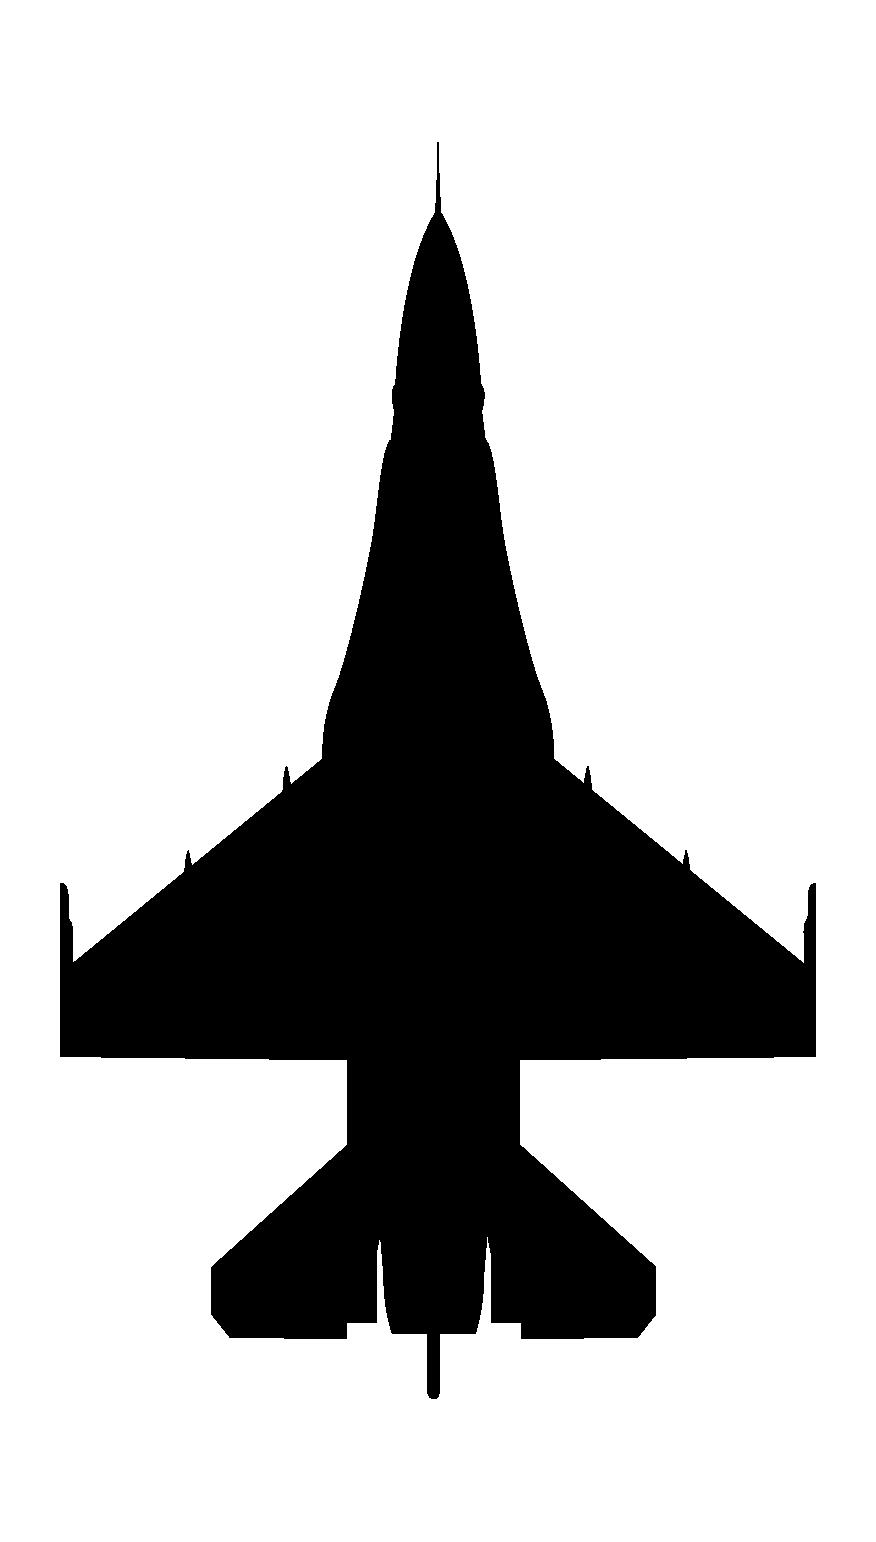
\includegraphics[
                width=7.5mm,
            ]{diagrams/aircraft/silhouette_f16_top.pdf}} 
            (naked_notch_start)
            arc (-180:-135:5) 
            -- ++(-45:15) 
            node[above, pos=1, rotate=-135] (naked_stagger_mid) {
                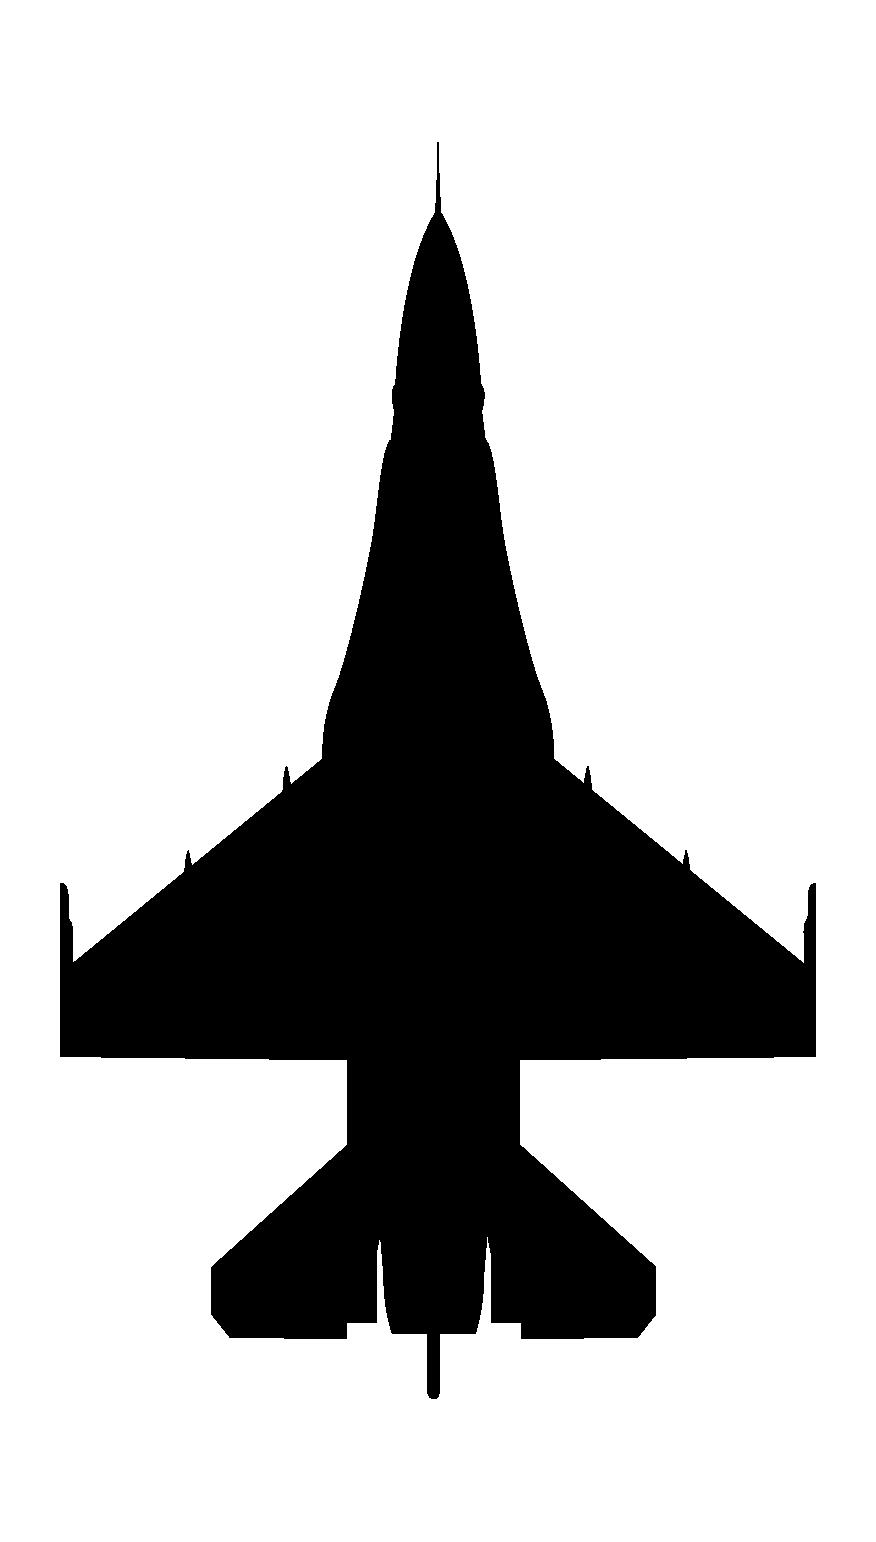
\includegraphics[
                    width=7.5mm,
                ]{diagrams/aircraft/silhouette_f16_top.pdf}
            };
        \draw[->]
            (naked_stagger_mid.north)
            arc (-135:30:5) 
            -- ++(120:20)
            node[above, pos=1, rotate=30] (naked_commit) {
                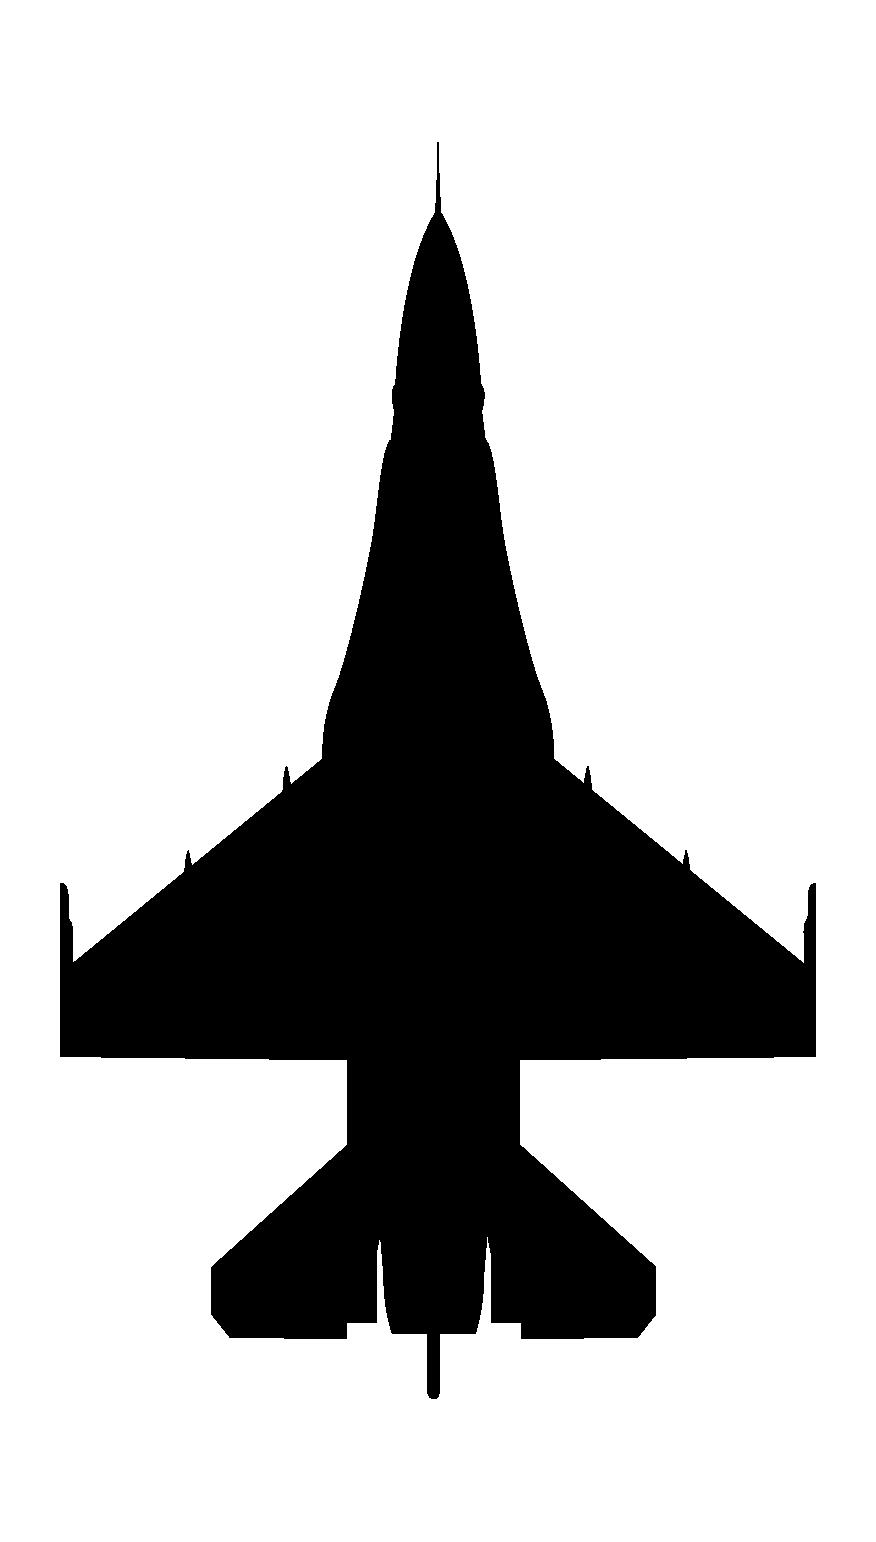
\includegraphics[
                    angle=0,
                    width=7.5mm,
            ]{diagrams/aircraft/silhouette_f16_top.pdf}};

        \node[font=\footnotesize, below] at (naked_stagger_mid.east) {Naked}; 
        \node[font=\footnotesize, right] at (naked_commit.east) {Commit};

        % spiked fighter
        \draw[->] 
            (spiked_start) -- 
            node[below, pos=0, rotate=180]{
                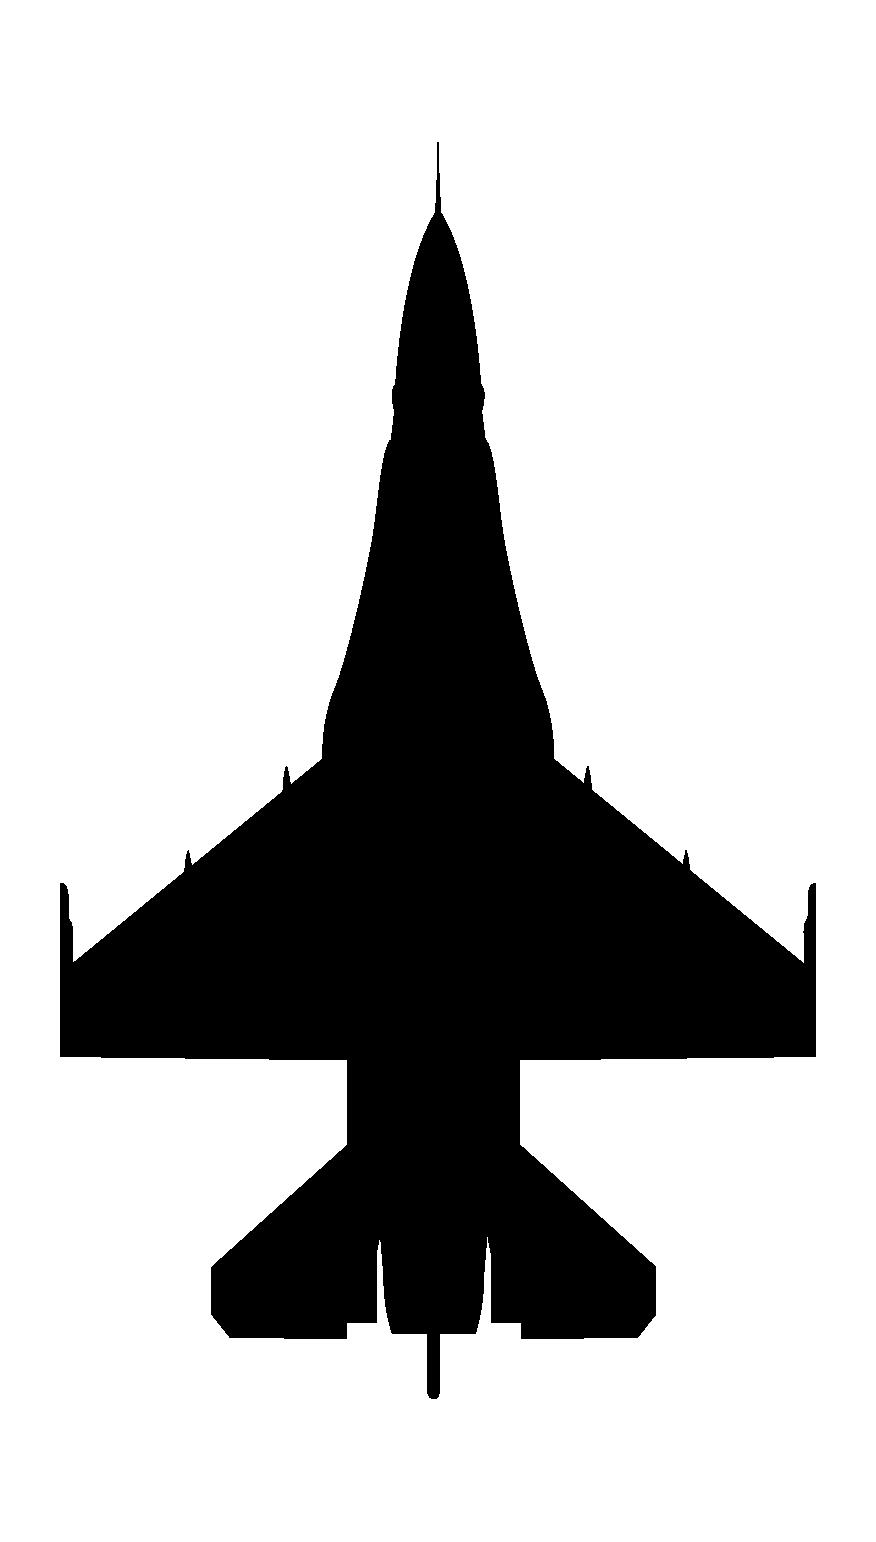
\includegraphics[
                width=7.5mm,
            ]{diagrams/aircraft/silhouette_f16_top.pdf}} 
            (spiked_notch_start)
            arc (0:-45:5) 
            -- ++(-135:15) 
            node[above, pos=1, rotate=135] (spiked_stagger_mid) {
                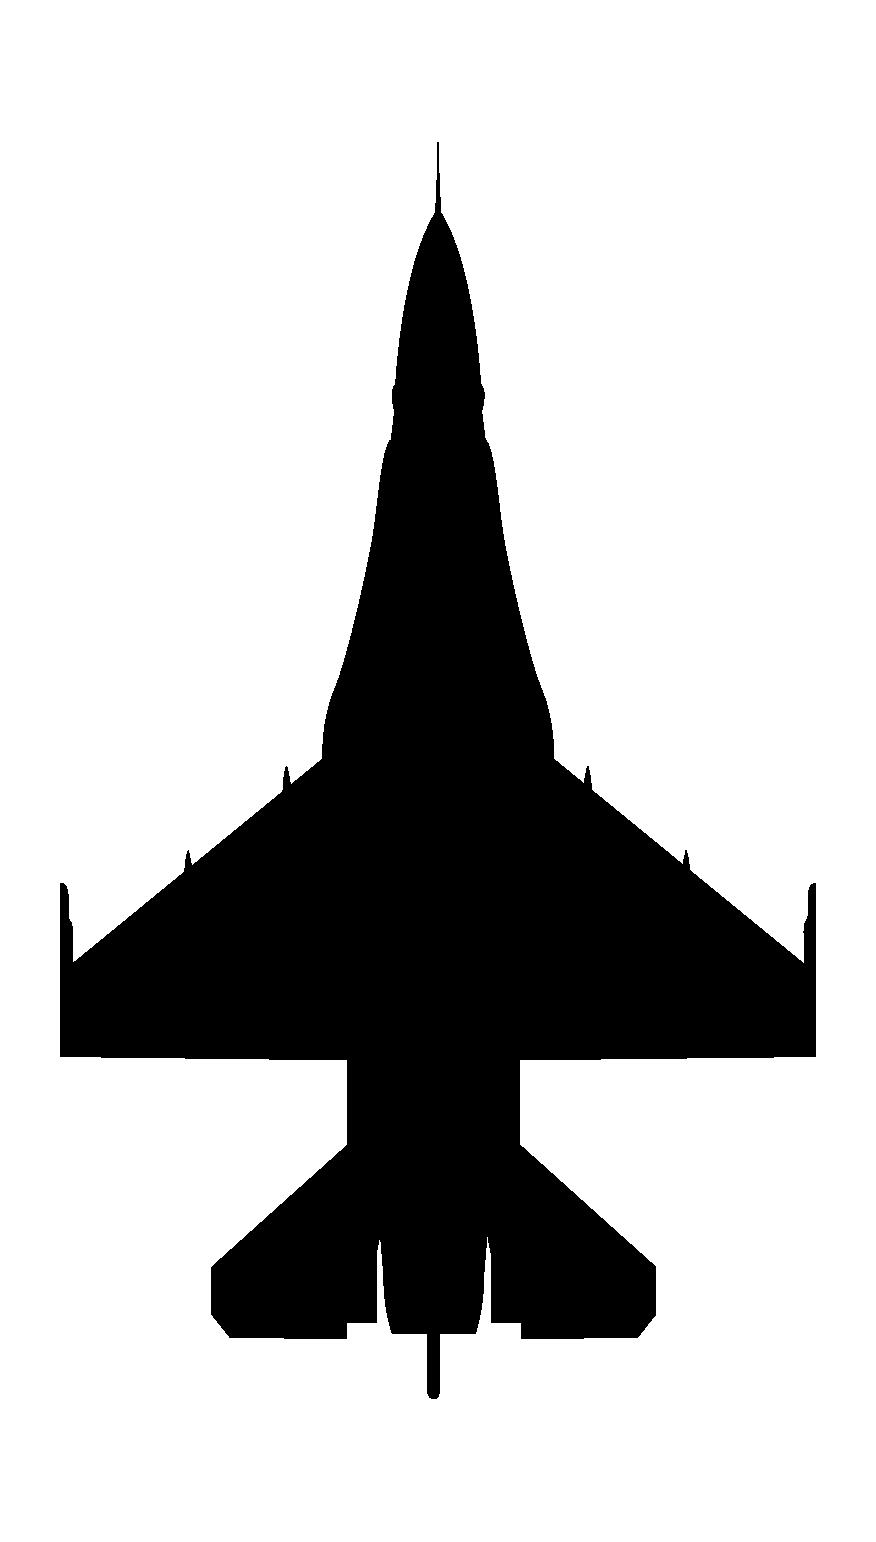
\includegraphics[
                    width=7.5mm,
                ]{diagrams/aircraft/silhouette_f16_top.pdf}
            };
        \draw[->]
            (spiked_stagger_mid.north)
            arc (135:180:5) 
            -- ++(0,-5)
            node[below, pos=1] (spiked_abort) {
                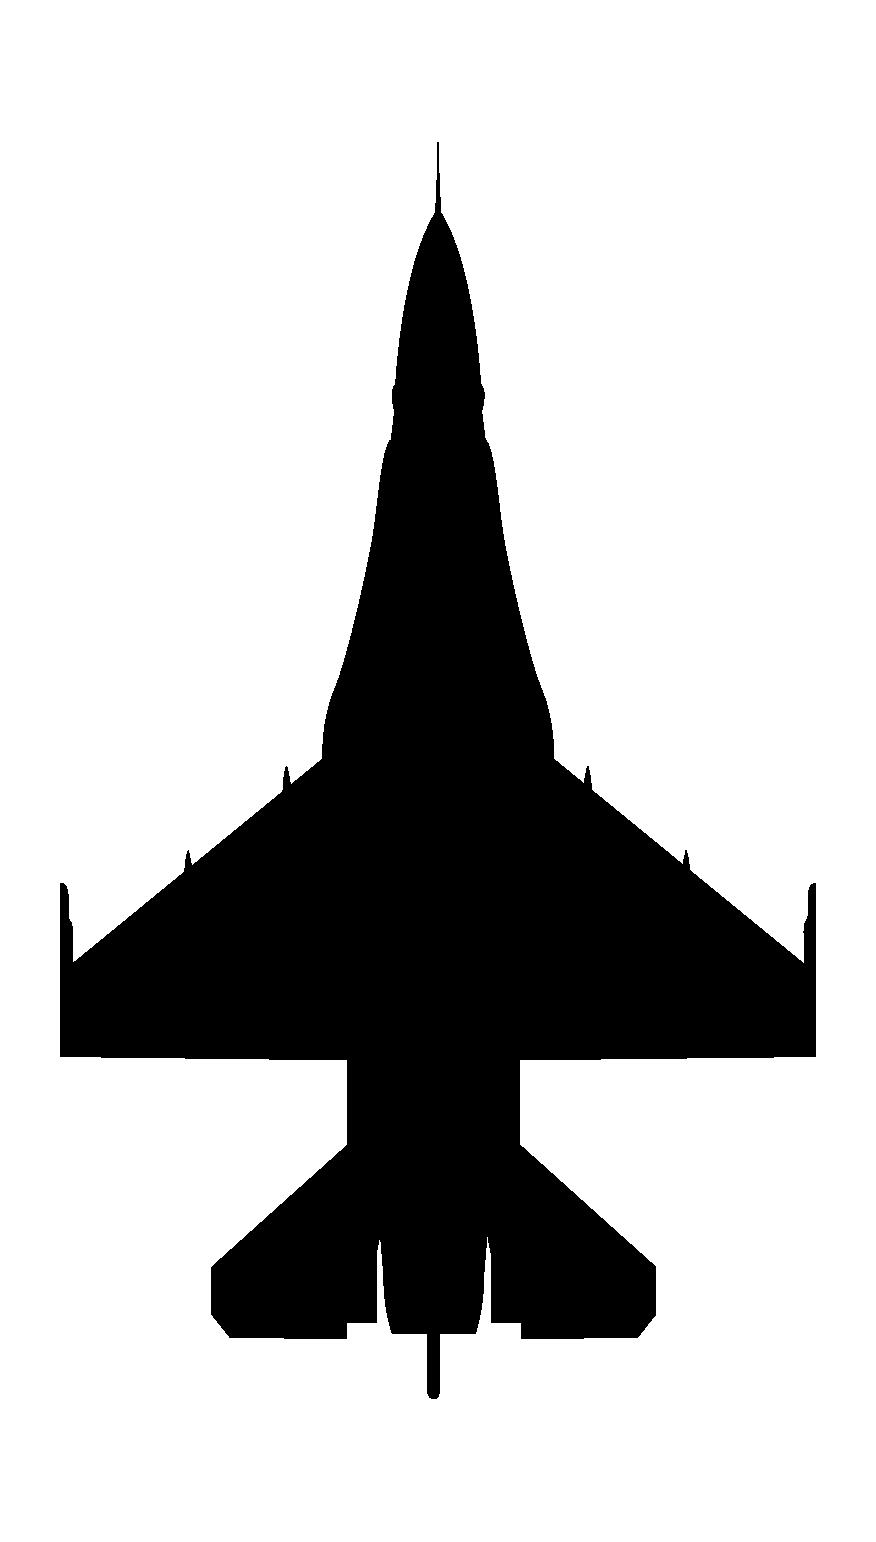
\includegraphics[
                    angle=180,
                    width=7.5mm,
            ]{diagrams/aircraft/silhouette_f16_top.pdf}};

        \node[font=\footnotesize, below] at (spiked_stagger_mid.west) {Spiked}; 
        \node[font=\footnotesize, below] at (spiked_abort.south) {Abort};

        % bandit
        \node[] at (bandit) {
            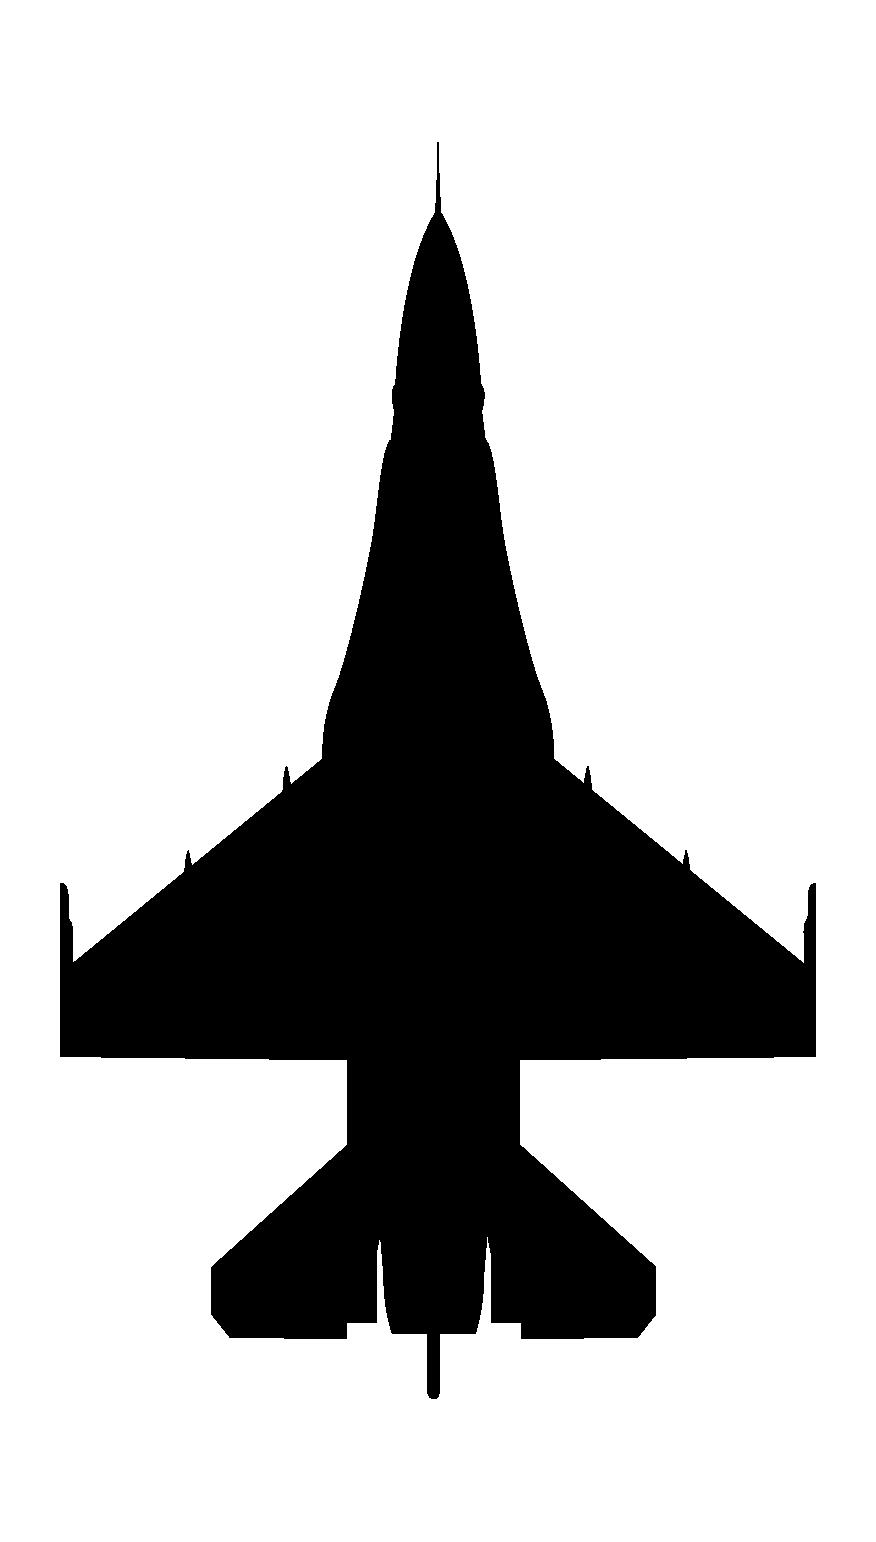
\includegraphics[
                angle=180,
                width=7.5mm,
        ]{diagrams/aircraft/silhouette_f16_top.pdf}};

    \end{tikzpicture}
    \caption{Stagger-back tactics}
    \label{fig:ttp_aa:element:offensive:staggerback}
\end{figure}

\begin{figure}[htbp]
    \centering
    \begin{tikzpicture}[figstyle]

        % coordinates
        \coordinate (naked_start) at (5,0);
        \coordinate (spiked_start) at (-5,0);
        \coordinate (bandit) at (0,45);

        \coordinate (naked_notch_start) at (5,-15);
        \coordinate (spiked_notch_start) at (-5,-15);

        % bandit wez
        \draw[fill=red!40]
            (bandit)
            -- ++(-105:72)
            arc (-105:-110:72)
            -- (bandit);

        \node[rotate=-90] (naked_notch_mid) at (20, -20) {
            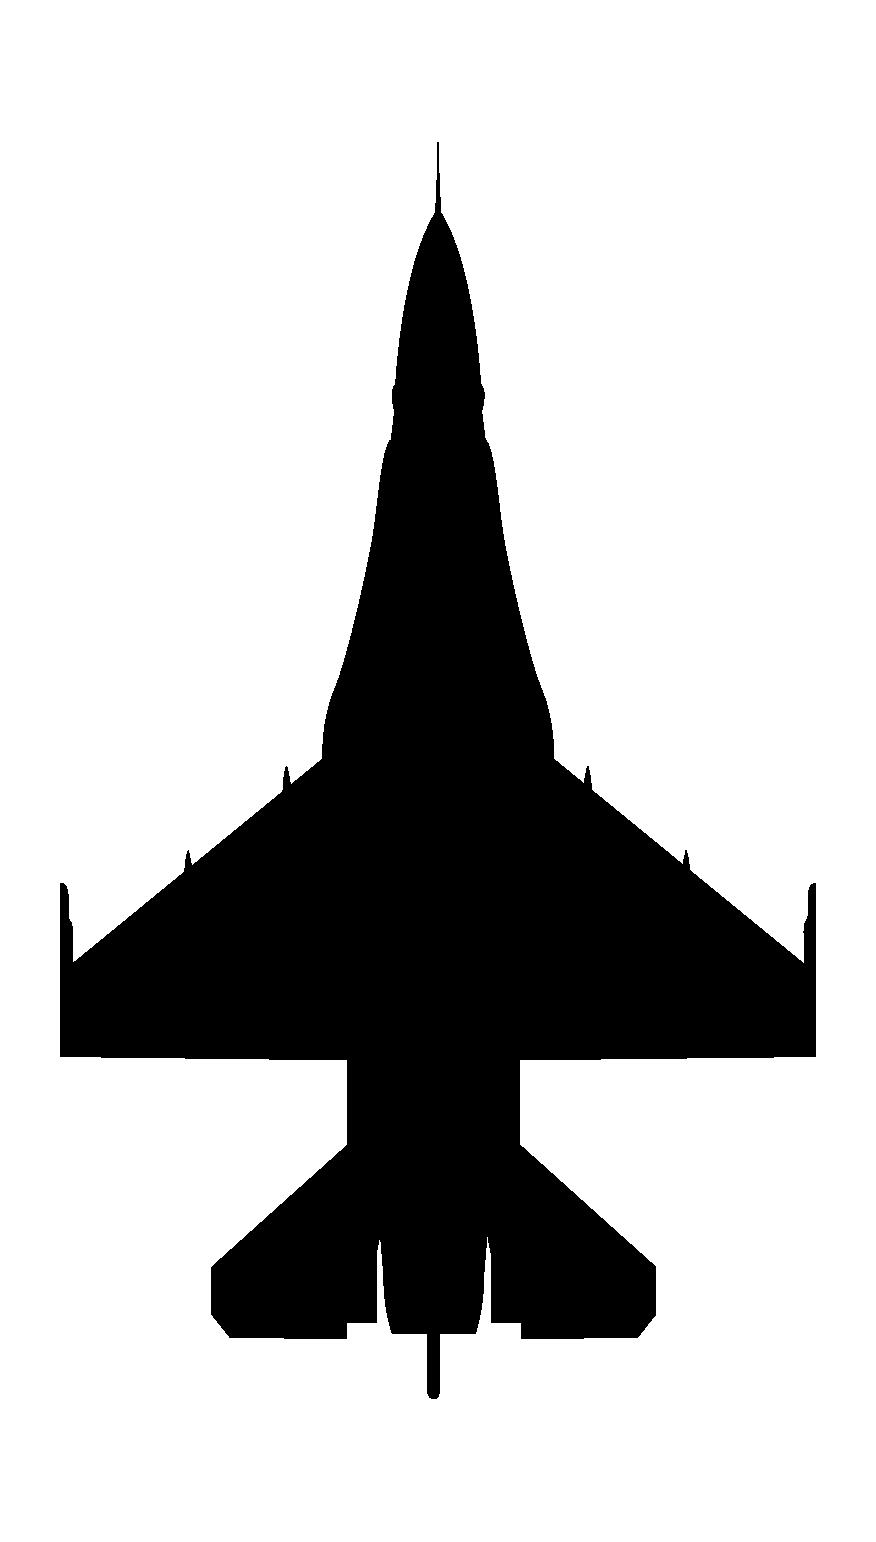
\includegraphics[
                width=7.5mm,
            ]{diagrams/aircraft/silhouette_f16_top.pdf}
        };
        \node[rotate=90] (spiked_notch_mid) at (-20, -20) {
            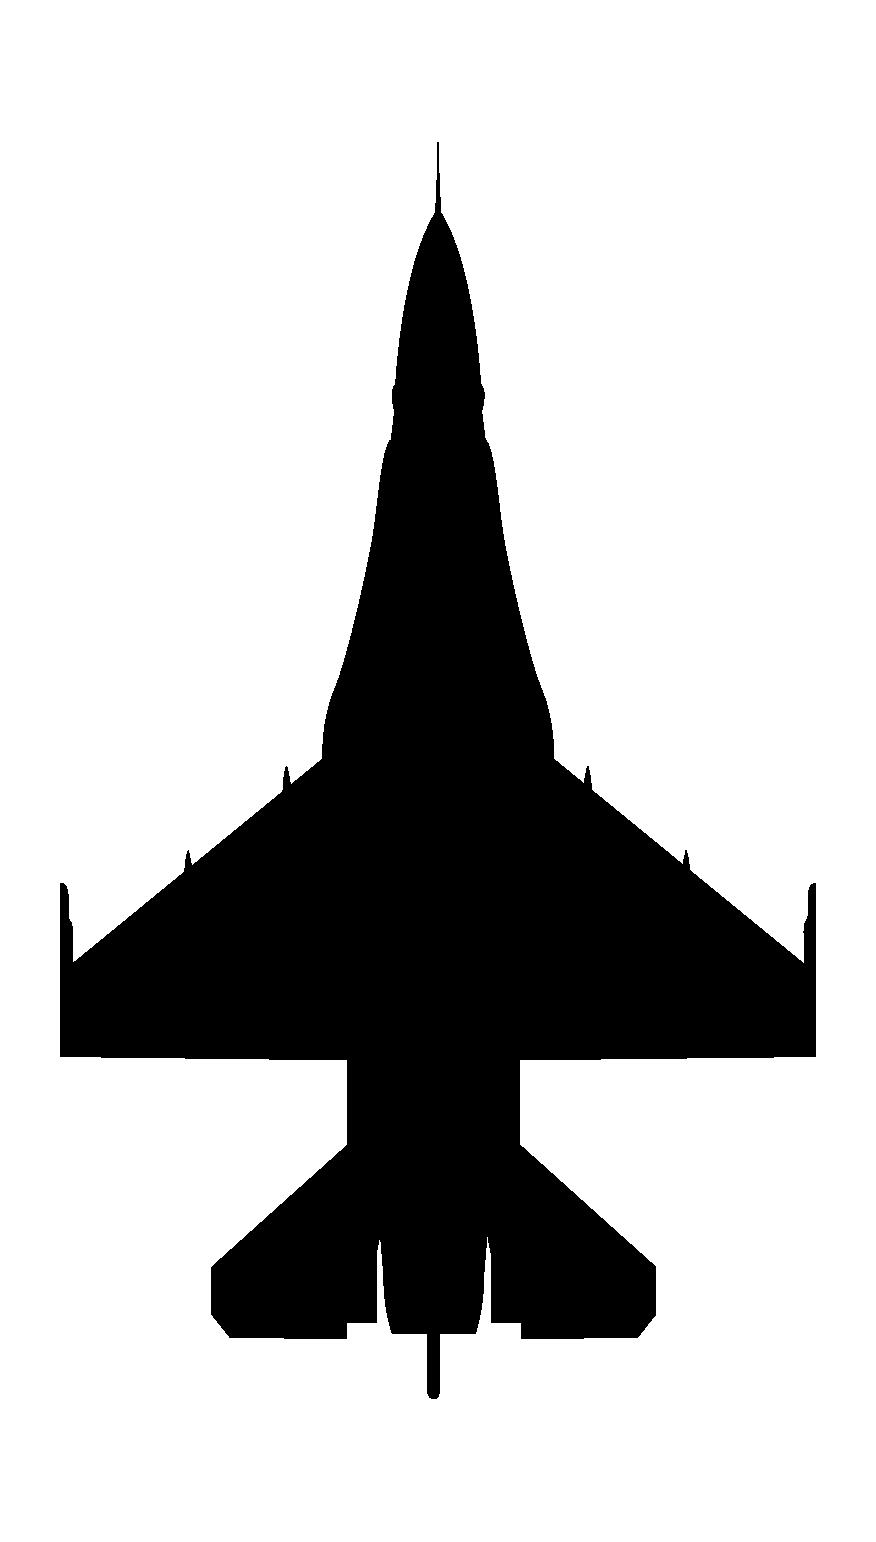
\includegraphics[
                width=7.5mm,
            ]{diagrams/aircraft/silhouette_f16_top.pdf}
        };
        
        % naked fighter
        \draw[->] 
            (naked_start) -- 
            node[below, pos=0, rotate=180]{
                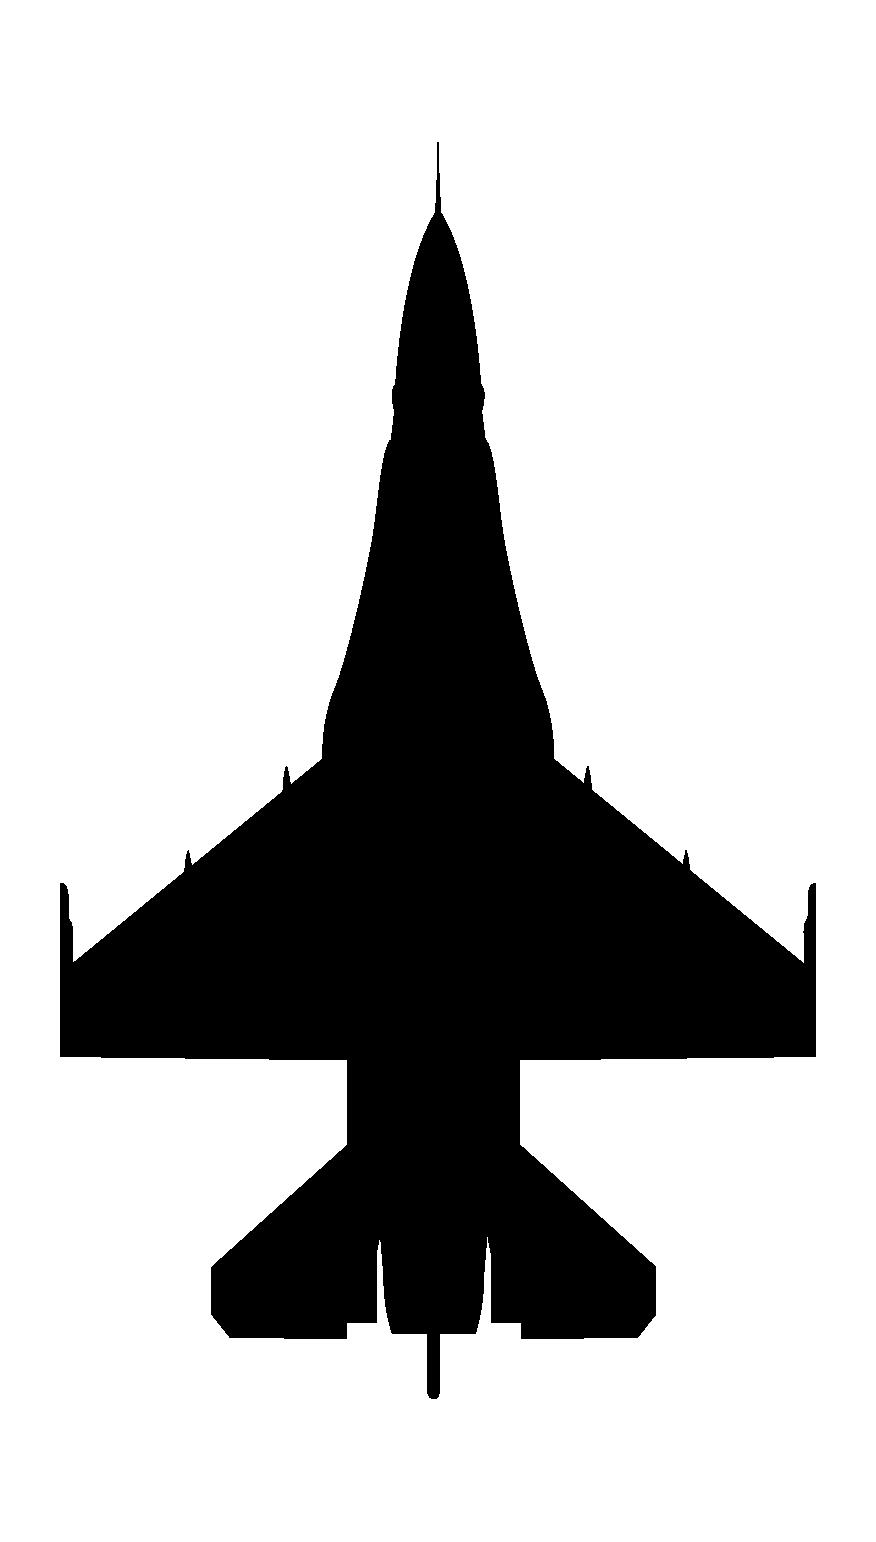
\includegraphics[
                width=7.5mm,
            ]{diagrams/aircraft/silhouette_f16_top.pdf}} 
            (naked_notch_start)
            arc (-180:-90:5) 
            -- (naked_notch_mid);
        \draw[->]
            (naked_notch_mid.north)
            arc (-90:30:5) 
            -- ++(120:10)
            node[above, pos=1, rotate=30] (naked_commit) {
                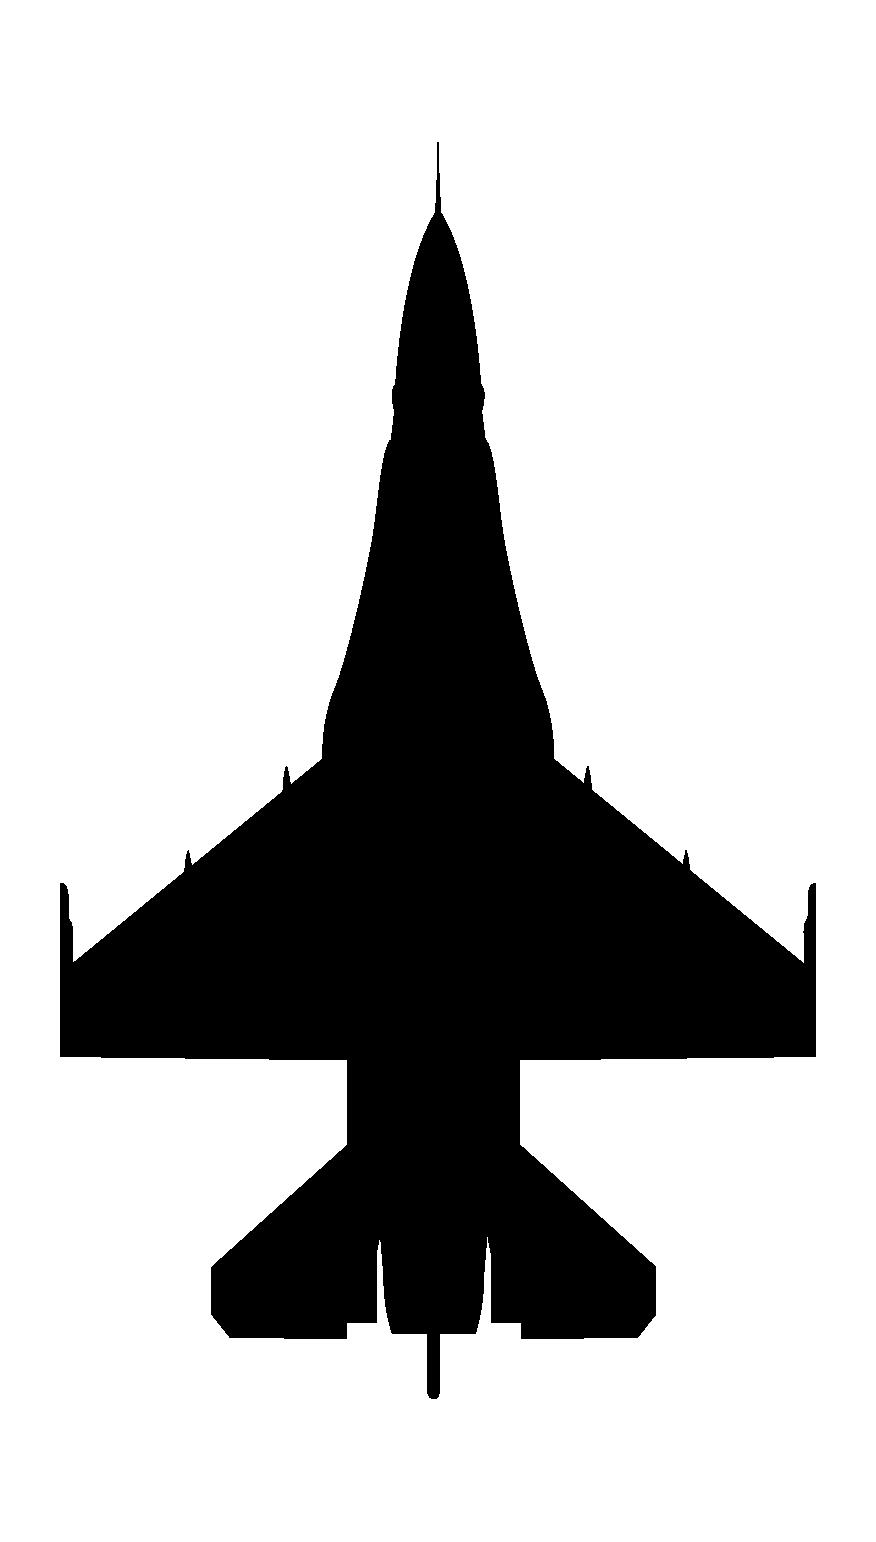
\includegraphics[
                    angle=0,
                    width=7.5mm,
            ]{diagrams/aircraft/silhouette_f16_top.pdf}};

        \node[font=\footnotesize, below] at (naked_notch_mid.east) {Naked}; 
        \node[font=\footnotesize, right] at (naked_commit.east) {Commit};

        % spiked fighter
        \draw[->] 
            (spiked_start) -- 
            node[below, pos=0, rotate=180]{
                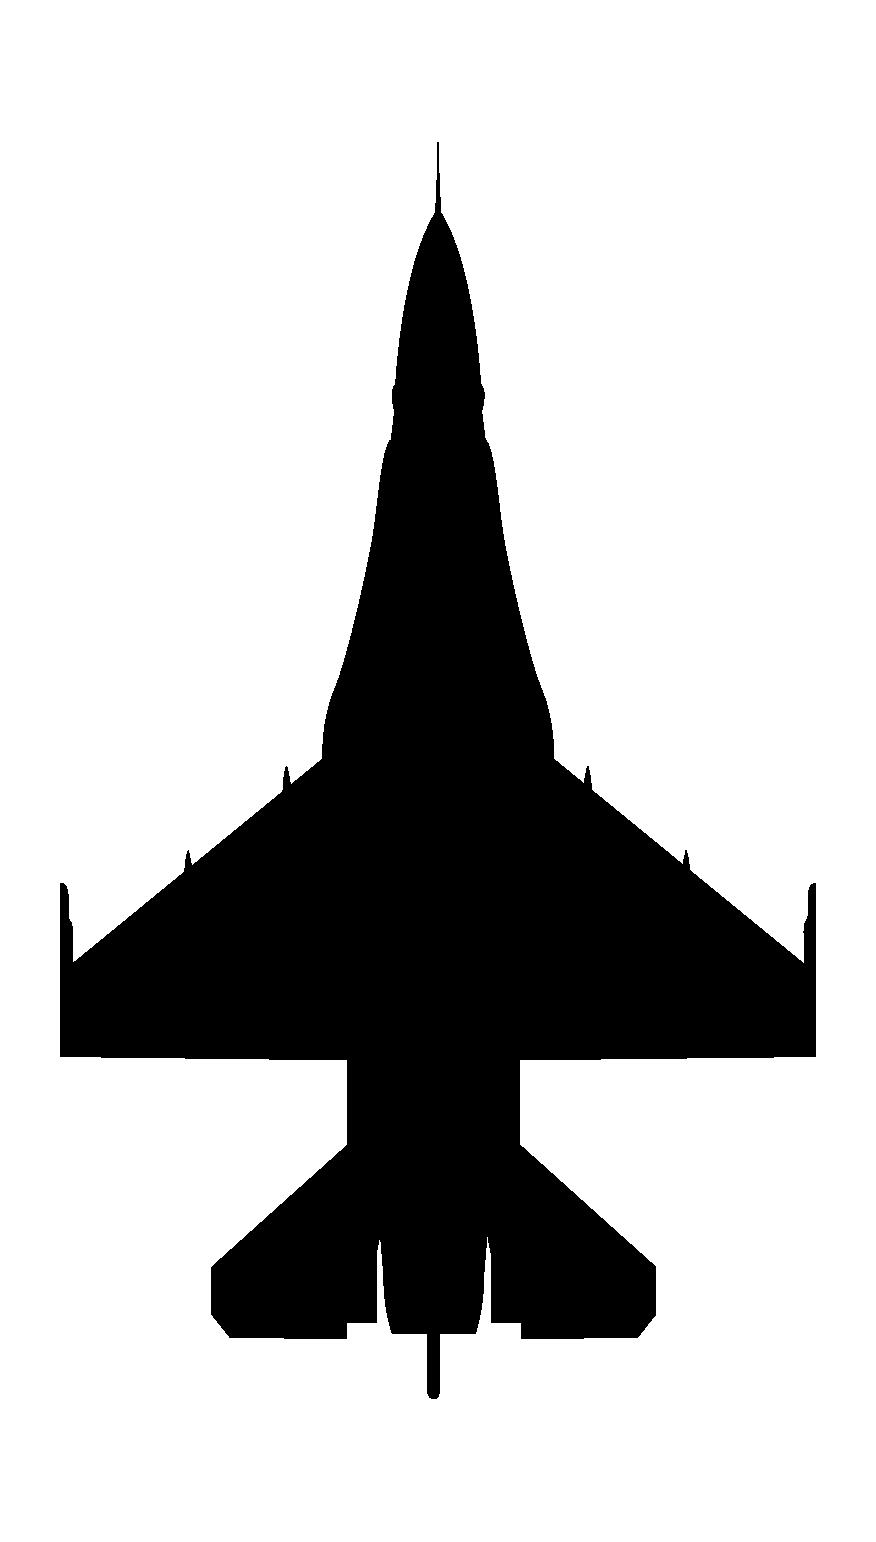
\includegraphics[
                width=7.5mm,
            ]{diagrams/aircraft/silhouette_f16_top.pdf}} 
            (spiked_notch_start)
            arc (0:-90:5) 
            -- (spiked_notch_mid);
        \draw[->]
            (spiked_notch_mid.north)
            arc (90:180:5) 
            -- ++(0,-5)
            node[below, pos=1] (spiked_abort) {
                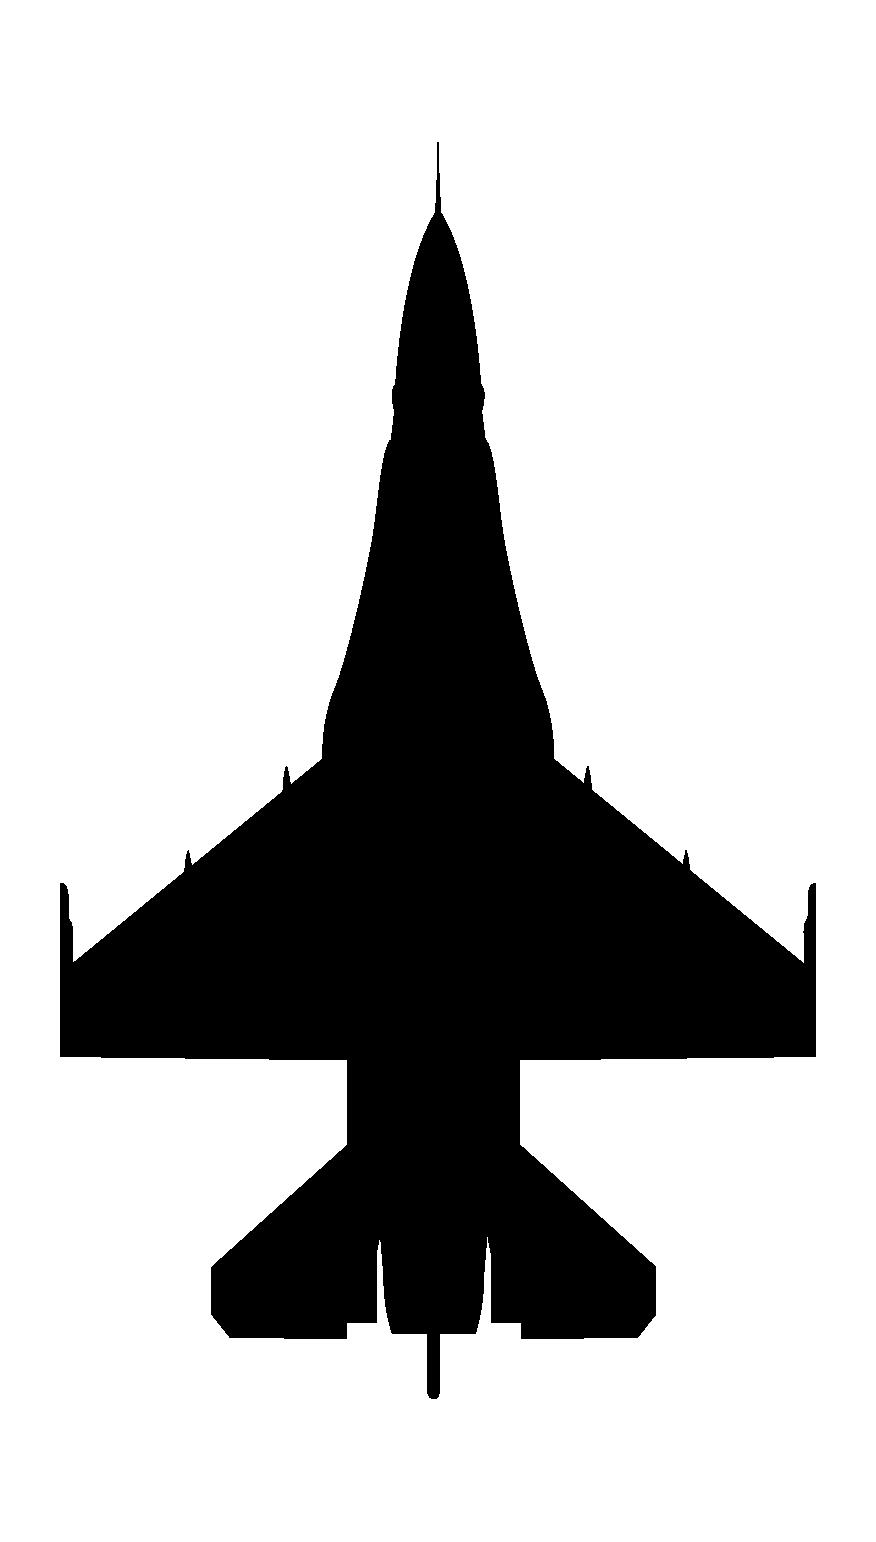
\includegraphics[
                    angle=180,
                    width=7.5mm,
            ]{diagrams/aircraft/silhouette_f16_top.pdf}};

        \node[font=\footnotesize, below] at (spiked_notch_mid.west) {Spiked}; 
        \node[font=\footnotesize, below] at (spiked_abort.south) {Abort};

        % bandit
        \node[] at (bandit) {
            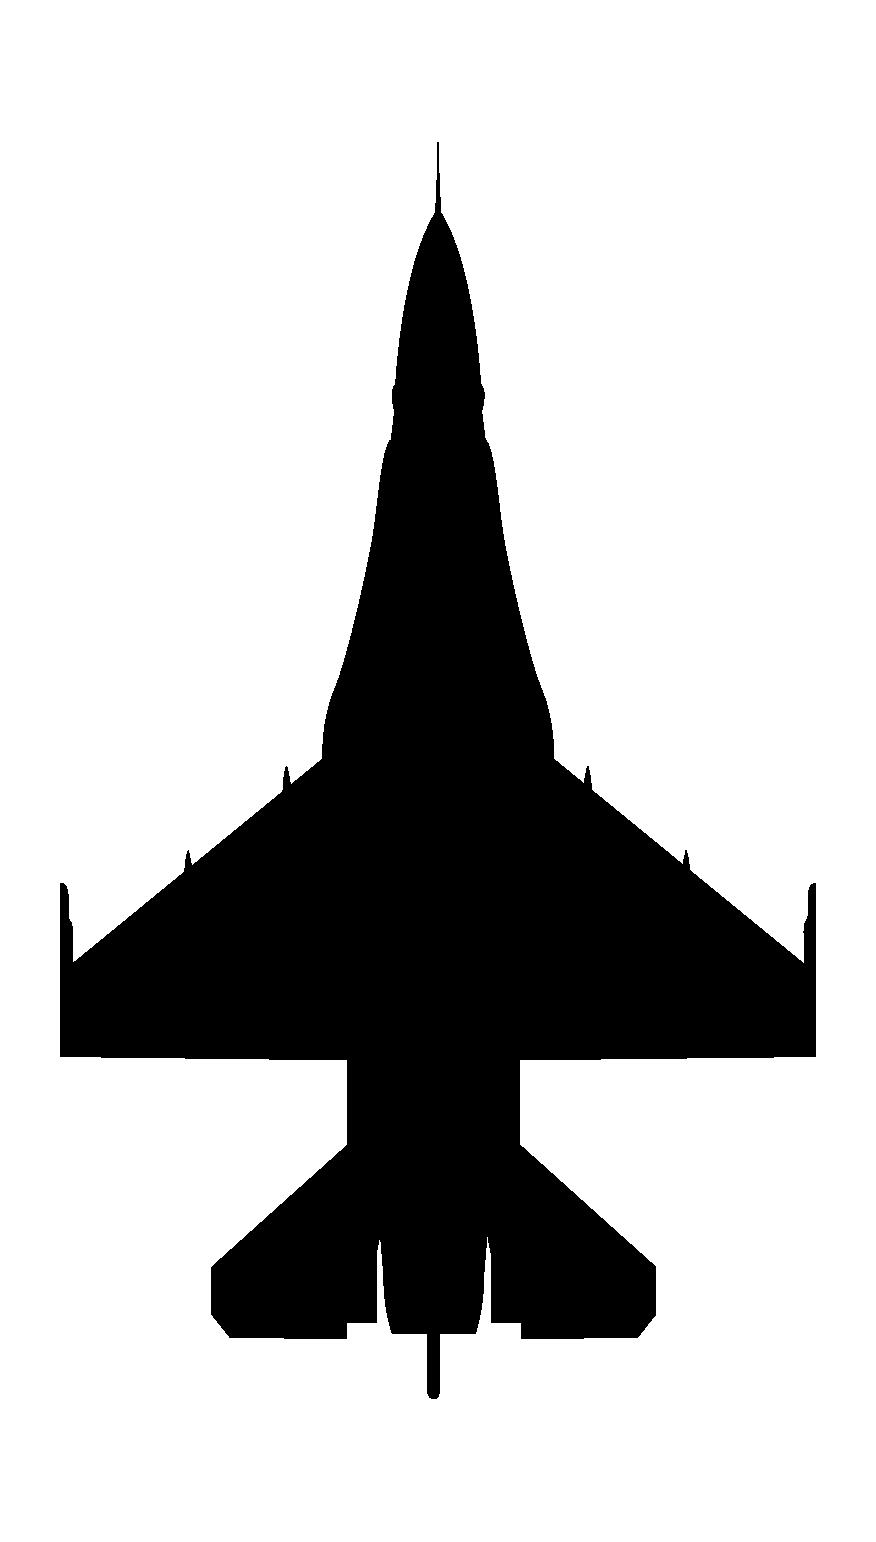
\includegraphics[
                angle=180,
                width=7.5mm,
        ]{diagrams/aircraft/silhouette_f16_top.pdf}};

    \end{tikzpicture}
    \caption{Notch-back tactics}
    \label{fig:ttp_aa:element:offensive:notchback}
\end{figure}

\clearpage